%!TEX root=main.tex
Our main idea is to model fairness using causal graphical models (CITE PEARL). Specifically we model observed feature(s) $X$, class label(s) $Y$, and sensitive attribute(s) $A$, as nodes in a directed acyclic graph (DAG). A directed arrow from any node $C$ to node $E$ indicates a causal relationship from cause $C$ to effect $E$. Mathematically, we take the approach of structural equation models as follows: if $C$ causes $E$ then $E$ is a function of $C$. Additionally, each node has an associated noise variable that are jointly independent


% and a noise variable associated with $C$, called $N_C$. (CITE) 


% a causal relation

%  where a directed arrow from


% that induce a joint distribution $P(X,Y,A)$. This distribution contains conditional independeces which can be expressed by a directed acyclic graph (DAG).









\begin{figure*}[th!]
\begin{center}
\vspace{-2ex}
\centerline{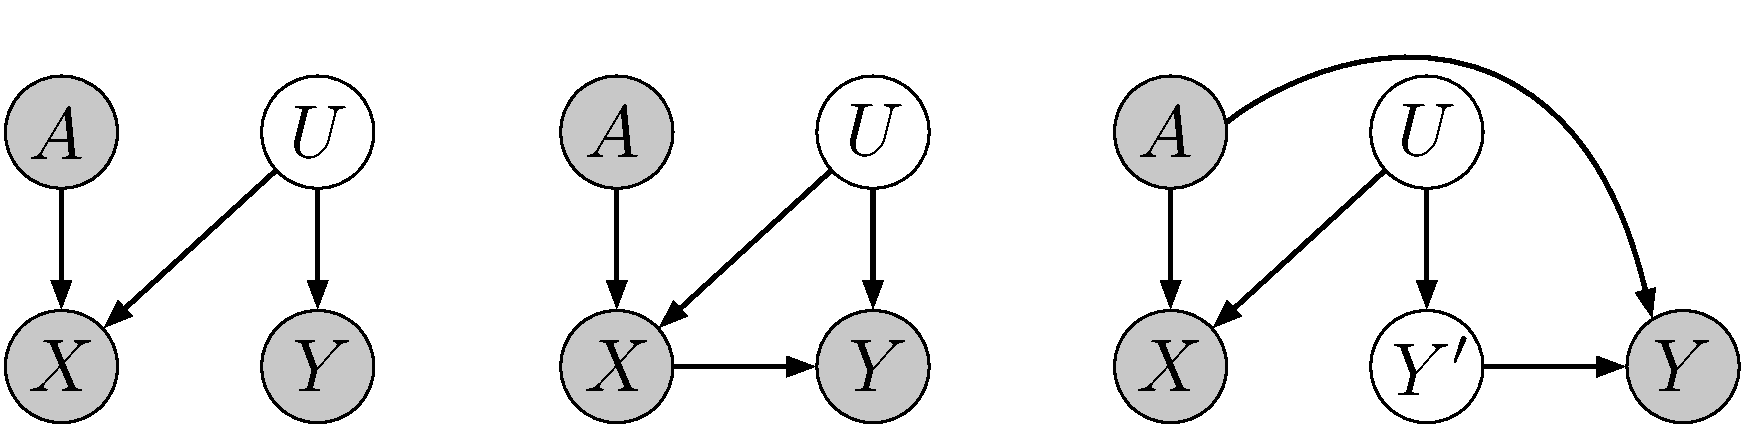
\includegraphics[width=\textwidth]{simple_models_no_q}}
\vspace{-2ex}
\caption{Three possible states of the world.\label{figure.simple_models}}
\vspace{-2ex}
\end{center}
\end{figure*}